\section{Introduction}
\label{sec:intro}

\begin{figure}[t]
  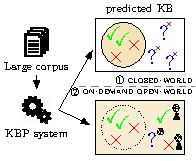
\includegraphics[width=\columnwidth]{figures/overview}
  \caption{\label{fig:overview}
  In knowledge base population (KBP), systems construct a knowledge base (KB) containing \textit{facts} about \textit{entities} 
  %such as where a person was born or who a company's founder is, 
  from a large document corpus documents.
  \encircle{1}
  Under the closed-world evaluation methodology, only those facts that intersect with the evaluation set of annotated facts
  %, usually constructed from other output of other systems,
  are considered to be true and all others are assumed false.
  %This can significantly penalize a novel system that predicts new facts outside what has already been annotated.
  \encircle{2}
  In the on-demand open-world methodology, predicted facts that have never been seen before are sampled and immediately annotated through crowd-sourcing to provide an unbiased estimate of performance in an open-world setting.
  }
\end{figure}

% (1 page w/ figure)
% Goal: remind the reader what information extraction is, what its relation to knowledge base population is and why it is important. Hook question.
% TODO: eh, make this shorter.
Harnessing the wealth of information present in troves of unstructured text has been and continues to be a long standing goal for the natural language processing community with many applications including question answering~\citep{berant2013freebase, fader2014open}, automated reasoning~\citep{kalyanpur2012structured} and dialogue~\citep{lee2015conversational,han2015exploiting}.
% TODO: better citations for ^^
%
% Evaluation @ scale poses problem.
However, evaluating such large-scale information extraction systems remains a challenge:
it is simply not economically feasible to exhaustively annotate every possible candidate fact from a sufficiently large corpus.
% TODO: am I doing justice to automatic evaluation peoples?
As a result, the community has adopted a heuristic wherein only a small evaluation set of annotated facts is used; predictions that intersect with this set are considered true, whereas all facts outside this ``closed-world'' are regarded to be false.
% TODO: Do I have a citation for CWA?
% Giving away the story a bit because it takes a little build up to really get into it.
In this work, we empirically show that the closed-world assumption can discourage innovation in the context of knowledge base population (KBP) and propose a solution that simulates access to a fully annotated ``open-world'' set of facts~(\figureref{overview}).

% II. 
% 1. KBP as case study -- what is KBP?
% TODO: is this too much detail?
%Before elaborating, let's look at how knowledge base population (KBP) is evaluated.
In KBP, a system is given a large document corpus and must output a knowledge base (KB) consisting of facts regarding which entities are mentioned in the corpus and how they are related, e.g.\ ``Carrie Fisher's mother is Debbie Reynolds'' or ``Carrie Fisher was born in Los Angeles'' (\figureref{task}). % according to a specified schema.
These predicted KBs are evaluated on how accurately they predict relations for an entity (precision) and how many of these relations they are able to correctly predict (recall), using an evaluation set and the closed-world assumption. %TODO: need a name for this set.

% III.
% 2. How is KBP evaluated? -- pooled eval, closed world assumption, output evaluated for a window.
The primary source of evaluation data for KBP comes from the annual TAC-KBP competition organized by NIST~\citep{}. % TODO: add links to workshop overview papers
Each year, teams submit their predicted KBs for a given document corpus.
Selected output is annotated by the organizers and released to help researchers develop better systems.
% TODO: while not biased for entrants in the competition, development sucks.
% - we measure pooling bias
Unfortunately, under the closed world assumption, new predictions that development systems make are not part of this evaluation data and are assumed to be wrong.\footnote according to our analysis.}
% - why it matters: effect on novel predictions -- hurts new ideas!
We estimate that this causes development \fone{} scores to be on average 2\% points lower than they should be, while significant improvements usually increase scores by less than 1\% \fone{}.
Worse yet, the more novel a system is, the stronger the bias against it will be, potentially even causing scores to drop.
% - while rule-based systems are robust because of human guidance -- empirically driven -- directs any output to what is already
While designers of rule-based systems can still look to their intuition for guidance, those who rely on empirical tuning and machine learning are, at best, left in the dark, and more likely to be directed towards only predicting what others have predicted and no more.
% - might explain great KBP stagnation -- bad scores and pattern based systems still leading -- cite system reports.
Of course, facts predicted by systems participating in the competition are fairly evaluated and do not suffer from any bias, but this requires researchers to wait a year to get credible feedback on new ideas.
%
These observations may explain why rule-based systems still play such a significant role in the top submissions at competition, and also as to why, even after 5 years of running the competition, top automated systems achieve scores of only about 35\%\fone{} while human annotators easily perform at \fake{60\%\fone{}}.

What, then, can be done to address this problem?
We propose a new evaluation framework in which predicted KBs submitted by researchers are suitably sampled and evaluated through crowd-sourcing.
The key challenges we must address are cost, ensuring coverage of entities and relations and ensuring unbiased estimates.
For the first, the framework leverages the fact that it is much cheaper to \textit{verify} facts than it is to find them within a large corpus.
For the second, we employ a structured sampling scheme to reduce the variance of entity-level and recall-level precision and recall.
Finally, we use exhaustive annotations for a few documents to de-bias our performance estimates in a cost-effective manner.

% I think pooling bias isn't necessarily what people will think of first, so moving this to related work / discussion.
% This ``pooling'' bias has also been identified in the information retrieval community\needcite, which bears many similarities to the knowledge base population task, e.g.\ both tasks seek to find ``relevant'' information from a large document corpus that is infeasible to exhaustively annotate.
% However, assessing the quality of system outputs is relatively objective in the context of knowledge base population.
% This enables us to employ non-expert crowdworkers to accurately judge novel output submitted by teams during development.

We simulate this framework on a mock evaluation of three distinct systems on the 2016 TAC-KBP corpus and find that we are able to estimate precision and recall within \fake{2\%} \fone{} (half as much as the official scores) and within a budget of \fake{\$2000} (a fraction of the cost of the official evaluation).
The framework and a public leaderboard will be made available at \url{http://anonymo.us}.
We hope to spur a new wave of progress on knowledge base population. 

\begin{figure}[t]
  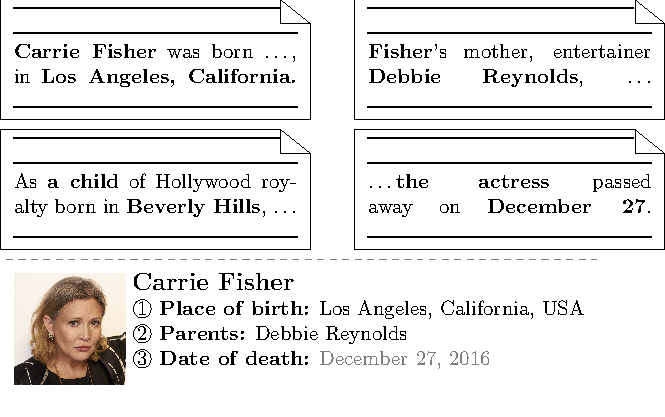
\includegraphics[width=\columnwidth]{figures/task}
  \caption{\label{fig:task}
  What do KBP outputs look like?
  }
\end{figure}

%integrating the output of several information extraction tasks, including entity detection and linking, relation extraction and event extraction.

% TODO: This line would be nice to follow, but it's pending a cross-year evaluation.
% Significant effort and resources have been invested in improving the performance of knowledge base population (KBP) systems, but have our systems actually gotten better and if so, by how much?

% Goal: Setup analysis by describing TAC-KBP. Describe first problem and how we solve it.
%The main way performance on the KBP task has been evaluated has been through the annual TAC-KBP competition organized by NIST.\@
%% TODO: argue the merits of the TAC-KBP challenge and its evaluation.
%The competition has invited more than \fake{300} submissions from at least \fake{40} different teams over the last 7 years (since 2009).
%Each year, teams are provided a document corpus and a list of query entities, for example ``Carrie Fisher'', to find facts for.
%The proposed facts from each participating team is pooled together and evaluated by human annotators.
%While scores of top performing teams have improved, they remain under \fake{35\% \fone}.
%In contrast, human evaluators provided access to simple text search for \fake{about 10 minutes} per query are able to identify far more facts and score about \fake{70\% \fone}.

%A number of confounding factors affect performance, including the performance of other systems, making comparisons difficult.
%This plateau should be alarming for any researcher; if we are to break through this ceiling, we need to understand better what is holding us back.
%Accordingly, we begin with an statistical analysis of the KBP evaluation in \sectionref{analysis}.
%Our key finding is that the evaluation data and methodology that teams use during development is actually biased against new features!
%We estimate that scores for new developments are on average 2\% points lower than they should be, a difference that can mask and even reverse the benefits of a new feature.

%The source of this bias arises because 
%the evaluation data only contains assessments for a subset of every candidate fact in the corpus
%and there is no good way to score a predicted fact that is not part of this subset.
%In particular, the evaluation data consists only of the candidate facts ``pooled'' together from systems that participated during the original competition and were subsequently assessed by human annotators.

%The platform is easy to use and will have a fresh stream of documents.

%For these reasons, we propose and implement a new evaluation methodology: an online evaluation platform that teams can submit to as they develop their systems (\sectionref{design}).
%We use a combination of exhaustive, selective and estimative annotations to balance cost, accuracy and guaranteed unbiased estimates of precision, recall and $\fone$ scores at the mention and entity level.
% \pl{I don't see the 'online evaluation platform' as the immediate solution;
% what I'd expect is a more technical solution - how to do the crowdsourcing to deal
% with bias and reweighting to deal with variance;
% making it online seems to help with more community aspects,
% which can be argued as valuable, but that seems like a separate point}

%\cite{chaganty2016perspectives}

%Next, we measure the effect of the pooling methodology \pl{need to explain pooling in enough detail for people to appreciate the problem} and find that it is significantly biased against unpooled systems: when evaluating improvements to your KBP system, your scores on the evaluation data could be 4--7\% lower than they would be if you had submitted said system; if you are developing a new KBP system, the bias can be as much as 20\%.
%This is serious methodological problem that provides a barrier of entry for new teams and makes incremental improvements to systems a coin toss-- real improvements in results will easily pass unnoticed. 


% We find that there is a large amount of variance in the scores due to varying difficulties of the query entities which leads to wide confidence intervals on the reported results.
% We show that this variance can be reduced by standardizing scores across queries, a new metric that is able to discriminate between systems \todo{50\%} more effectively. 
% \pl{the variance doesn't seem to be the thing causing the plateau;
% certainly it doesn't explain the difference between 30\% and 80\%;
% seems the bias is more pressing and should be talked about first
% }


% TODO: We haven't tried doing a cross-evaluation yet -- this would basically mean we take a reference system and try and compare performance across years relative to this system.
% We use a method for score standarization (\refsec{analysis}) to compare scores across years and find that \todo{there is no statistically significant improvement in the last several years}.

